{ \large \bfseries 2.Περιγραφή της Σχεδίασης}\\ % title 2

\begin{justify}
    Το κύριο χαρακτηριστικό του \textlatin{pipeline} 
    επεξεργαστή είναι ότι εκτελεί πολλές εντολές ταυτόχρονα
    σε έναν κύκλο του ρολογιού, σε αντίθεση με τους
    \textlatin{single} και \textlatin{multi}
    \textlatin{cycle} επεξεργαστές οπου για να ξεκινήσει
    μια νέα εντολή πρέπει πρώτα να έχει ολοκληρωθεί η τρέχουσα.
\end{justify}

\begin{justify}
    Η αρχή της λειτουργίας του \textlatin{pipeline} επεξεργαστή
    μοιάζει πολύ με αυτή του \textlatin{multi-cycle} ως προς
    το ότι βασίζεται στον διαχορισμό της εκτέλεσης σε
    στάδια τα όποία είναι όμοια με τα στάδια του 
    \textlatin{multi-cycle}:
\end{justify}

\begin{center}
    {\bf \textlatin{IF\_stage} / \textlatin{DEC\_stage} /
    \textlatin{EXEC\_stage} / \textlatin{MEM\_stage} /
    \textlatin{WB\_stage} }
\end{center}

\begin{justify}
    Για να γίνει το παραπάνω, τοποθετήθηκαν καταχωρητές
    μεταξύ των 5 σταδίων που αποθηκεύουν όλες τις
    εξόδους που παράγονται από το κάθε στάδιο και
    περνάνε σαν εισόδους στο επόμενο. Ακόμη, τοποθετήθηκαν
    καταχωρητές και για τα \textlatin{control} σήματα
    ώστε να μη χάνεται η πληροφορία που χρειάζονται οι εντολές
    για να λειτουργήσουν όταν περνάνε από το ένα στάδιο στο
    επόμενο. Όλοι οι απαραίτητοι καταχωρητές έχουν ομαδοποιθεί
    στα εξής \textlatin{modules} (για λόγους ιεραρχικής σχεδίασης):
\end{justify}

\begin{center}
    {\bf \textlatin{IF\_DEC} / \textlatin{DEC\_EX} /
    \textlatin{EX\_MEM} / \textlatin{MEM\_WB} }
\end{center}

\begin{justify}
    Για την αντιμετώπιση των \textlatin{datahazards} 
    δημιουργήθηκαν το {\bf \textlatin{Forwarding Unit}}
    και το {\bf \textlatin{Hazard Detection Unit}}. 
    Στην περίπτωση του \textlatin{Forwarding Unit}, 
    \textlatin{hazard} μπορεί να προκύψει όταν η τιμή ενός
    καταχωρητή του \textlatin{Register File} χρειαστεί σε 
    μια επόμενη εντολή (αφού οι εντολές εκτελούνται ταυτόχρονα,
    δε θα έχουν προλάβει να ολοκληρωθούν οι 5 κύκλοι εκτέλεσης).
    Αφού πργαμοτοποιηθούν (σύμφωνα με την θεωρία) οι απαραίτητοι
    έλεγχοι και επιβεβαιωθεί ότι υπάρχει \textlatin{hazard},
    δίνουμε την κατάλληλη εισόδο στον \textlatin{Register File} 
    χωρίς να περιμένουμε αυτή να βγει από το \textlatin{WB\_stage}.
\end{justify}

\begin{justify}
    Στην περίπτωση του {\bf \textlatin{Hazard Detection Unit}},
    επιτυγχάνεται η αντιμετώπιση των \textlatin{datahazards}
    μέσω \textlatin{stalls}. Σε αυτή την περίπτωση, όταν
    ένας καταχωρητης παίρνει τιμή από την μνήμη,
    πρέπει αναγκαστικά να περάσει και από τα 5 στάδια εκτέλεσης,
    οπότε αμα χρησιμοποιείται από μια επόμενη εντολή, αυτή
    πρέπει να περιμένει. Μόλις ανισχνευθεί \textlatin{hazard},
    παγώνουν τα \textlatin{IF\_stage} και \textlatin{DEC\_stage}
    απενεργοποιώντας τα \textlatin{write enable} των κατάληλλων
    καταχωρητών και εισάγοντας μηδενικά στην βαθμίδα σημάτων
    ελέγχου του \textlatin{DEC\_EX}.
\end{justify}


\newpage

\begin{justify}
    Ακολουθεί \textlatin{Block Diagram} της ολοκληρωμένης σχεδίασης:
\end{justify}


\begin{figure}[h]
    \raggedright
    \hspace{-1cm}
    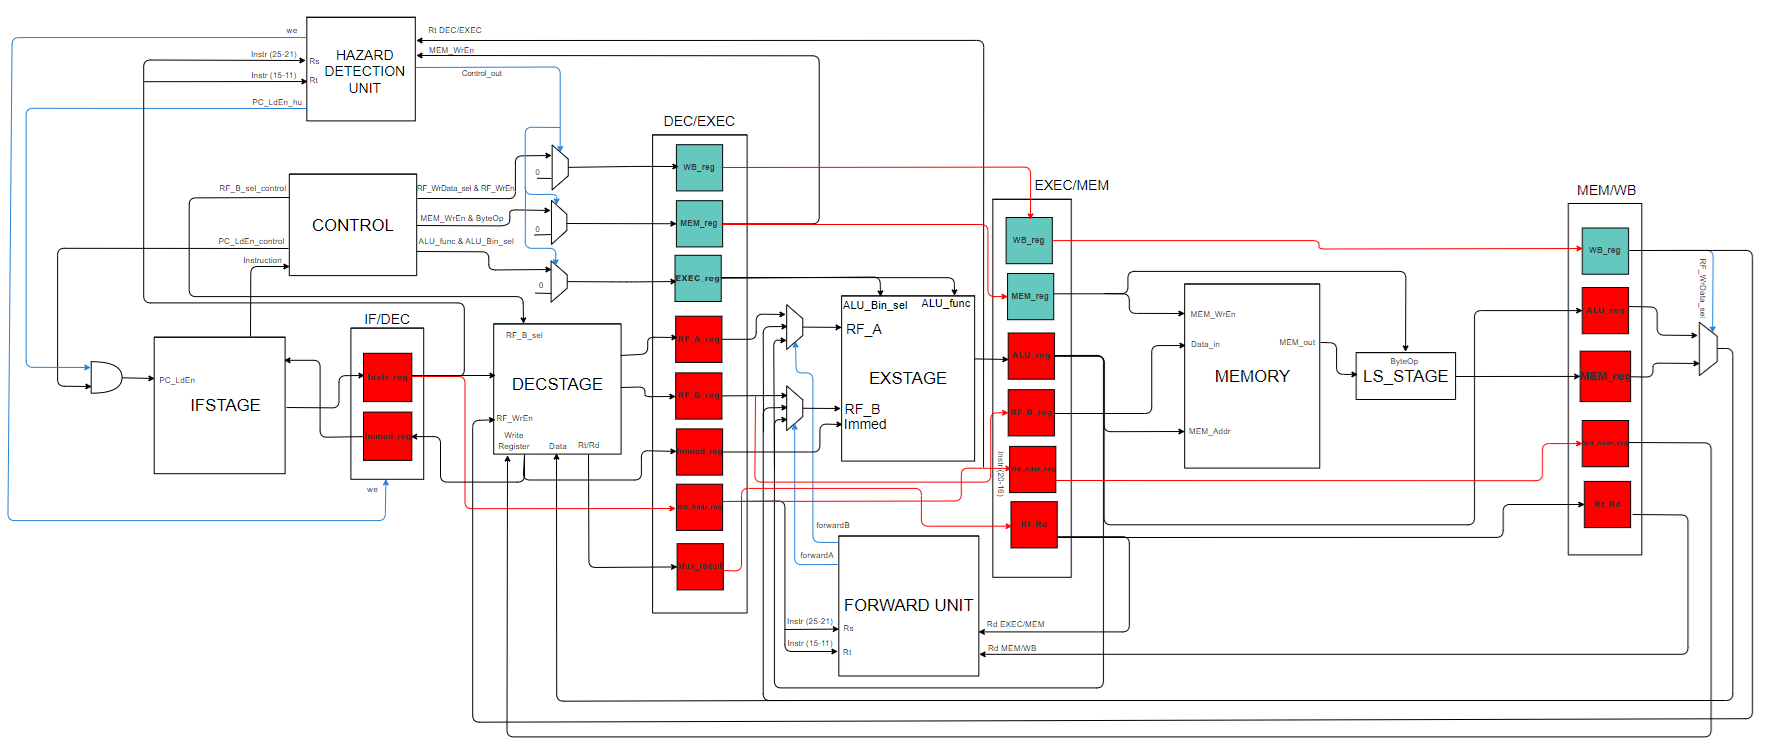
\includegraphics[width=1.1\textwidth]{IMAGES/BLOCK_DIAGRAM.png} % Adjust width as needed
\end{figure}